\documentclass{article}
\usepackage{amsmath, amsthm}
\usepackage{tikz}
\usetikzlibrary{arrows.meta, positioning, shapes, patterns}

\newtheorem{theorem}{Theorem}
\newtheorem{definition}{Definition}

\begin{document}

\section{The P3 Wind Tunnel: Synthetic Validation of USLA Dynamics}

\subsection{Introduction: The Architect's Proving Ground}

The Unified State and Logic Architecture (USLA) represents a complete formalization of system dynamics, from the atomic state vector, \(x_t\), to the universal laws of state transition, \(\Delta p\). While the architecture is mathematically sound on paper, any real-world implementation is subject to the complexities of code, environment, and unforeseen interactions.

P3 is our proving ground. It is a high-fidelity "wind tunnel" designed for a single purpose: to simulate and validate the pure, internal dynamics of a USLA-compliant system. By abstracting away all external dependencies, P3 allows us to observe the raw mathematical evolution of the state vector under the influence of its own physics engine (\(\Delta p\)). It is the final, synthetic crucible where we verify that our implementation faithfully executes the logic of the architectural blueprint before exposing it to the unpredictable currents of reality.

\subsection{The Simulation Core: State, Physics, and Law}

At its heart, P3 is a sophisticated discrete-time simulation loop that models three fundamental components:

\begin{description}
    \item[The State Vector (\(x_t\))] This is a comprehensive, high-dimensional vector that represents a perfect, instantaneous snapshot of the entire system at a moment in time, \(t\). It contains every piece of information necessary to define the system's condition—from configuration parameters and operational states to logical assertions and accumulated metrics.
    
    \item[The Transition Engine (\(\Delta p\))] The \(\Delta p\) engine is the system's heart. It is a deterministic function that computes the change in the state vector for a single time step. Given the current state \(x_t\), the engine applies the complete set of USLA physics to produce a delta, such that the next state is defined as \(x_{t+1} = x_t + \Delta p(x_t)\). This engine is the codified embodiment of all the rules, heuristics, and corrective forces that govern the system's behavior.
    
    \item[USLA Laws & \(\Omega\) Constraints] The \(\Delta p\) engine does not operate in a vacuum. Its calculations are strictly bounded by the foundational USLA laws and the system's specific operational envelope, defined by \(\Omega\) (Omega) constraints. These are the immutable "laws of physics" for the simulation, ensuring that every state transition is valid, coherent, and aligned with the system's fundamental principles of integrity and stability.
\end{description}

\begin{figure}[h!]
\centering
% TikZ Diagram 1: The P3 Simulation Loop
\begin{tikzpicture}[
    node distance=2.5cm,
    block/.style={rectangle, draw, fill=blue!10, text width=8em, text centered, rounded corners, minimum height=4em},
    law/.style={rectangle, draw, fill=green!10, text width=8em, text centered, rounded corners, minimum height=4em},
    line/.style={draw, -{Stealth[length=2mm]}}
]
    \node [block] (state) {System State \(x_t\)};
    \node [block, right=of state] (engine) {\(\Delta p\) Physics Engine};
    \node [law, below=of engine] (laws) {USLA Laws & \(\Omega\) Constraints};
    \node [block, above=of engine] (state_next) {System State \(x_{t+1}\)};

    \path [line] (state) -- node[above] {Compute} (engine);
    \path [line] (laws) -- (engine);
    \path [line] (engine) -- node[above, text width=6em] {\(x_{t+1} = x_t + \Delta p(x_t)\)} (state_next);
    \path [line] (state_next) .. controls +(up:1cm) and +(up:1cm) .. (state);
\end{tikzpicture}
\caption{The core iterative loop of the P3 simulation.}
\end{figure}

\subsection{Mathematical Guarantees: Robbins-Monro Convergence}
The P3 simulation is more than a procedural check; it is the physical realization of a powerful class of mathematical theorems that guarantee system stability and convergence. The dynamics of USLA are engineered to conform to the principles of \textbf{stochastic approximation}, pioneered by Robbins and Monro.

The \(\Delta p\) engine is designed to provide a noisy but unbiased estimate of the gradient of a performance landscape (e.g., maximizing the Reality-Serviceability Index, or RSI). Each iteration of the P3 loop is a step in the direction of this estimated gradient. The \textbf{Robbins–Siegmund Theorem} provides the crucial guarantee that such a process, under general conditions that USLA is designed to meet, will almost surely converge to a stable equilibrium.

\begin{figure}[h!]
\centering
% TikZ Diagram 2: The Convergence Landscape
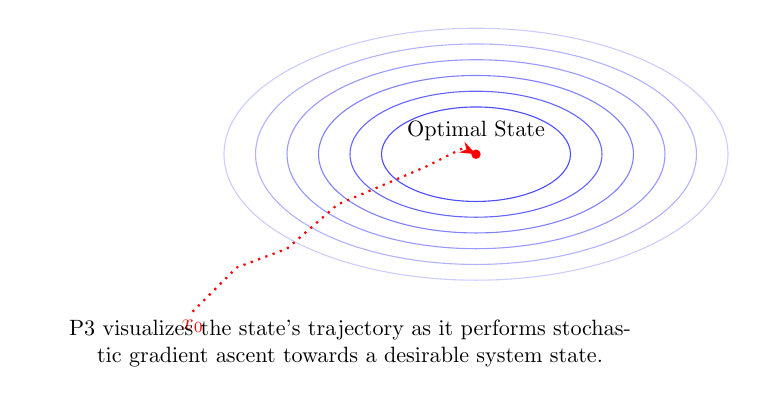
\begin{tikzpicture}[scale=0.8, every node/.style={transform shape}]
    % Contour lines
    \draw[blue!20] (0,0) ellipse (4cm and 2cm);
    \draw[blue!30] (0,0) ellipse (3.5cm and 1.75cm);
    \draw[blue!40] (0,0) ellipse (3cm and 1.5cm);
    \draw[blue!50] (0,0) ellipse (2.5cm and 1.25cm);
    \draw[blue!60] (0,0) ellipse (2cm and 1cm);
    \draw[blue!70] (0,0) ellipse (1.5cm and 0.75cm);

    % Peak
    \node at (0,0) [circle, fill=red, inner sep=1.5pt, label=above:{Optimal State}] {};

    % Path
    \draw[red, thick, dotted, -{Stealth[length=2mm]}] 
        (-4.5, -2.5) node[below] {\(x_0\)}
        -- (-3.8, -1.8) -- (-3.0, -1.5) -- (-2.2, -0.8) 
        -- (-1.5, -0.5) -- (-0.8, -0.2) -- (-0.2, 0.1) -- (0,0);
    
    \node at (-2, -3) [text width=10cm, text centered] 
    {P3 visualizes the state's trajectory as it performs stochastic gradient ascent towards a desirable system state.};
\end{tikzpicture}
\caption{The Convergence Landscape.}
\end{figure}

\subsection{Limitations: The Model-Reality Gap}
For all its power, the P3 wind tunnel has a fundamental limitation: it can only validate the model, not reality. A successful P3 run provides high confidence that the system's internal logic is sound, stable, and implemented correctly. It proves that, given a starting state \(x_0\), the system will evolve exactly as the laws of USLA predict. However, it makes no claim about how well \(x_0\) and the \(\Delta p\) physics represent the actual, messy, and unpredictable real world.

\begin{figure}[h!]
\centering
% TikZ Diagram 3: The Map and the Territory
\begin{tikzpicture}[
    panel/.style={rectangle, draw, thick, minimum height=5cm, minimum width=5cm}
]
    % Left Panel: The Map
    \node[panel, label=above:{\textbf{The Map: P3 Simulation}}] (map) at (-3,0) {};
    \begin{scope}[shift={(map.center)}, scale=0.35]
        \draw[blue!20] (0,0) ellipse (4cm and 2cm);
        \draw[blue!40] (0,0) ellipse (3cm and 1.5cm);
        \draw[blue!60] (0,0) ellipse (2cm and 1cm);
        \node at (0,0) [circle, fill=red, inner sep=1.5pt] {};
        \draw[red, thick, dotted, -{Stealth[length=1.5mm]}] (-4.5, -2.5) -- (-3, -1.5) -- (-1, -0.5) -- (0,0);
    \end{scope}

    % Right Panel: The Territory
    \node[panel, label=above:{\textbf{The Territory: The Real World}}] (territory) at (3,0) {};
     \begin{scope}[shift={(territory.center)}, scale=0.35]
        \fill[gray!20, pattern=north east lines, pattern color=gray!40] (-4.5,-3) rectangle (4.5,3);
        \draw[black!50, thick, jagged] (-4, -2) -- (-2, 1) -- (0, -1) -- (1, 2) -- (3, -1.5) -- (4, 1);
        \node at (1.5,2.5) [cloud, draw, fill=white] {Fog};
        \draw[-{Stealth[length=3mm]}, red, thick] (0.5, 2.5) -- (0, 1.5) node[below] {Shock};
     \end{scope}

    % Arrow
    \draw[dashed, -{Stealth[length=4mm]}, line width=1.5pt] (map.east) -- (territory.west) node[midway, above] {Deployment};
\end{tikzpicture}
\caption{P3 certifies the internal logic of the map; correspondence with the territory requires empirical validation.}
\end{figure}

\newpage

\appendix
\section{Mathematical Appendix Draft}

\begin{definition}[State Vector \(x_t\)]
Let \(S\) be the state space of the system. The state vector \(x_t \in S \subset \mathbb{R}^n\) is a vector that completely describes the system at discrete time \(t\). It is a concatenation of sub-vectors representing configuration, operational parameters, logical states, and performance metrics:
\[ x_t = [c_t, o_t, l_t, m_t]^T \]
where \(c_t\) are configuration parameters, \(o_t\) are operational variables, \(l_t\) are logical assertions (e.g., boolean flags), and \(m_t\) are accumulated metrics like RSI.
\end{definition}

\begin{definition}[The \(\Delta p\) Map]
The transition engine is a deterministic map \(\Delta p: S \to \mathbb{R}^n\) that computes the state update. The evolution of the system is given by the discrete-time dynamical system:
\[ x_{t+1} = x_t + \alpha_t \cdot \Delta p(x_t, \xi_t) \]
Here, \(\alpha_t\) is a sequence of positive step sizes, and \(\xi_t\) represents a stochastic element or noise term, which in P3 is synthetically generated to simulate search over the state space. The function \(\Delta p\) is engineered such that it approximates the gradient of a hidden performance function \(f(x)\), i.e., \(\mathbb{E}[\Delta p(x, \xi)] \approx \nabla f(x)\).
\end{definition}

\begin{theorem}[Robbins-Siegmund Conditions for USLA]
The USLA framework and the \(\Omega\) constraints ensure the conditions for the Robbins-Siegmund Theorem are met for the sequence \(x_t\). Let \((\mathcal{F}_t)\) be the filtration generated by the process. We require:
\begin{enumerate}
    \item \textbf{Boundedness:} The state is confined to a compact set \(\Omega \subset S\), i.e., \(x_t \in \Omega\) for all \(t\). This is enforced by the USLA constraint system.
    \item \textbf{Step Size Conditions (Robbins-Monro):} The step sizes \(\alpha_t\) must satisfy:
    \[ \sum_{t=1}^{\infty} \alpha_t = \infty \quad \text{and} \quad \sum_{t=1}^{\infty} \alpha_t^2 < \infty \]
    A common choice is \(\alpha_t = 1/t\).
    \item \textbf{Supermartingale Property:} The process must be a "nearly-supermartingale" with respect to some Lyapunov-like function \(V(x_t)\), ensuring that on average, each step does not move "uphill" away from the desired state. For our purposes, where we are maximizing \(f(x)\), the process \(-f(x_t)\) should have this property.
\end{enumerate}
\end{theorem}

\begin{definition}[Convergence Claim]
Under the conditions above, the sequence \(x_t\) generated by the P3 simulation will converge almost surely to the set of stationary points of \(f(x)\) within \(\Omega\). That is,
\[ \lim_{t \to \infty} \nabla f(x_t) = 0 \quad \text{a.s.} \]
This provides a strong guarantee that the P3 simulation will find a stable, high-performance equilibrium point, validating the correctness of the implemented \(\Delta p\) physics.
\end{definition}

\end{document}
